\section{Definição}

\begin{frame}[fragile]{Definição}

    \begin{itemize}
        \item A travessia por largura (\textit{Breadth-First Search -- BFS}) visita os nós
            em ordem crescente em relação à distância entre estes nós e o nó inicial $s$

        \item Desta forma, um subproduto da BFS é a distância de todos os nós que estão conectados 
            até $s$

        \item A implementação da BFS é mais trabalhosa do que a da DFS, porque não se vale de
            recursão, sendo necessário o uso de uma fila explicitamente

        \item Ambas travessias visitam os mesmos nós, porém em ordens distintas

        \item A complexidade da BFS é $O(N + M)$, onde $N$ é o número de vértices e $M$ o 
            número de arestas do grafo conectado

        \item No caso de uma representação por matrizes de adjacência, a complexidade é
            $O(N^2)$
    \end{itemize}

\end{frame}

\begin{frame}[fragile]{Visualização da BFS}

    \begin{tikzpicture}
        \node[anchor=west] at (0,0) { Fila: 1 };
        \draw (0,4) -- (2,6);
        \draw (0,4) -- (2,2);
        \draw (2,6) -- (4,7);
        \draw (2,6) -- (4,5);
        \draw (4,5) -- (4,3);
        \draw (4,3) -- (2,2);
        \draw (4,3) -- (4,1);
        \draw (4,3) -- (6,2);
        \draw (4,5) -- (6,6);
        \draw (4,5) -- (6,4);
        \draw (6,2) -- (6,4);
        \draw (6,6) -- (8,5);
        \draw (8,5) -- (8,3);
        \draw (8,5) -- (10,4);

        \node[circle, draw, fill=white] at (0, 4) {1};
        \node[circle, draw, fill=white] at (2, 6) {2};
        \node[circle, draw, fill=white] at (2, 2) {3};
        \node[circle, draw, fill=white] at (4, 7) {4};
        \node[circle, draw, fill=white] at (4, 5) {5};
        \node[circle, draw, fill=white] at (4, 3) {6};
        \node[circle, draw, fill=white] at (4, 1) {7};
        \node[circle, draw, fill=white] at (6, 6) {8};
        \node[circle, draw, fill=white] at (6, 4) {9};
        \node[circle, draw, fill=white] at (6, 2) {10};
        \node[circle, draw, fill=white] at (8, 5) {11};
        \node[circle, draw, fill=white] at (8, 3) {12};
        \node[circle, draw, fill=white] at (10, 4) {13};

    \end{tikzpicture}

\end{frame}

\begin{frame}[fragile]{Visualização da BFS}

    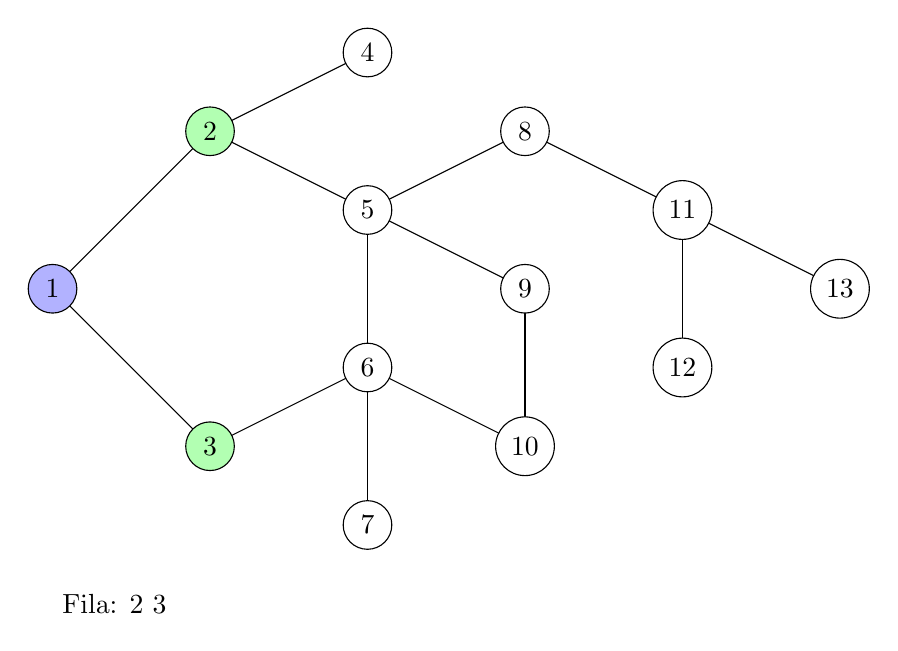
\begin{tikzpicture}
        \node[anchor=west] at (0,0) { Fila: 2 3 };
        \draw (0,4) -- (2,6);
        \draw (0,4) -- (2,2);
        \draw (2,6) -- (4,7);
        \draw (2,6) -- (4,5);
        \draw (4,5) -- (4,3);
        \draw (4,3) -- (2,2);
        \draw (4,3) -- (4,1);
        \draw (4,3) -- (6,2);
        \draw (4,5) -- (6,6);
        \draw (4,5) -- (6,4);
        \draw (6,2) -- (6,4);
        \draw (6,6) -- (8,5);
        \draw (8,5) -- (8,3);
        \draw (8,5) -- (10,4);

        \node[circle, draw, fill=blue!30] at (0, 4) {1};
        \node[circle, draw, fill=green!30] at (2, 6) {2};
        \node[circle, draw, fill=green!30] at (2, 2) {3};
        \node[circle, draw, fill=white] at (4, 7) {4};
        \node[circle, draw, fill=white] at (4, 5) {5};
        \node[circle, draw, fill=white] at (4, 3) {6};
        \node[circle, draw, fill=white] at (4, 1) {7};
        \node[circle, draw, fill=white] at (6, 6) {8};
        \node[circle, draw, fill=white] at (6, 4) {9};
        \node[circle, draw, fill=white] at (6, 2) {10};
        \node[circle, draw, fill=white] at (8, 5) {11};
        \node[circle, draw, fill=white] at (8, 3) {12};
        \node[circle, draw, fill=white] at (10, 4) {13};

    \end{tikzpicture}

\end{frame}

\begin{frame}[fragile]{Visualização da BFS}

    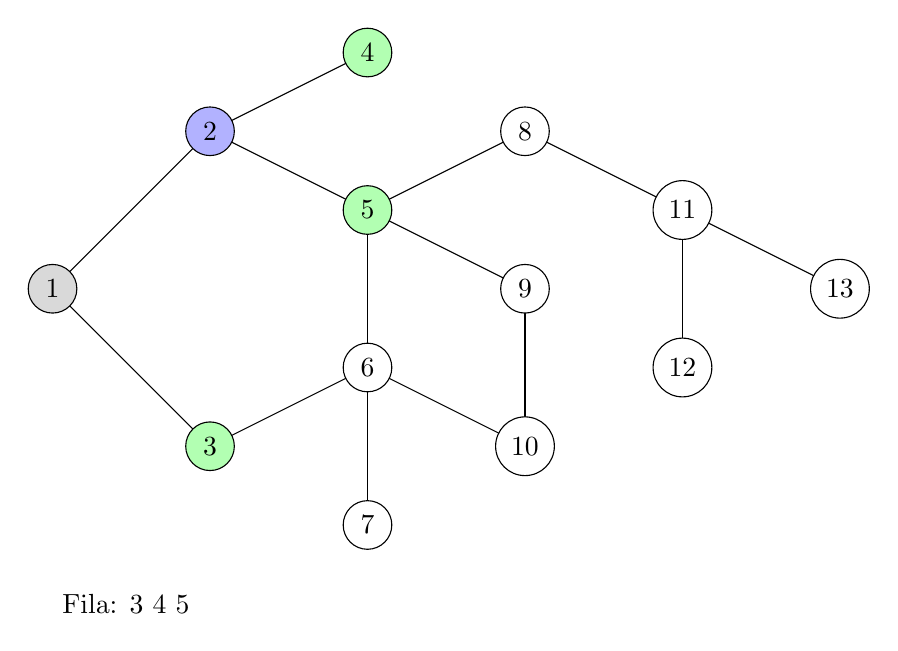
\begin{tikzpicture}
        \node[anchor=west] at (0,0) { Fila: 3 4 5 };
        \draw (0,4) -- (2,6);
        \draw (0,4) -- (2,2);
        \draw (2,6) -- (4,7);
        \draw (2,6) -- (4,5);
        \draw (4,5) -- (4,3);
        \draw (4,3) -- (2,2);
        \draw (4,3) -- (4,1);
        \draw (4,3) -- (6,2);
        \draw (4,5) -- (6,6);
        \draw (4,5) -- (6,4);
        \draw (6,2) -- (6,4);
        \draw (6,6) -- (8,5);
        \draw (8,5) -- (8,3);
        \draw (8,5) -- (10,4);

        \node[circle, draw, fill=gray!30] at (0, 4) {1};
        \node[circle, draw, fill=blue!30] at (2, 6) {2};
        \node[circle, draw, fill=green!30] at (2, 2) {3};
        \node[circle, draw, fill=green!30] at (4, 7) {4};
        \node[circle, draw, fill=green!30] at (4, 5) {5};
        \node[circle, draw, fill=white] at (4, 3) {6};
        \node[circle, draw, fill=white] at (4, 1) {7};
        \node[circle, draw, fill=white] at (6, 6) {8};
        \node[circle, draw, fill=white] at (6, 4) {9};
        \node[circle, draw, fill=white] at (6, 2) {10};
        \node[circle, draw, fill=white] at (8, 5) {11};
        \node[circle, draw, fill=white] at (8, 3) {12};
        \node[circle, draw, fill=white] at (10, 4) {13};

    \end{tikzpicture}

\end{frame}

\begin{frame}[fragile]{Visualização da BFS}

    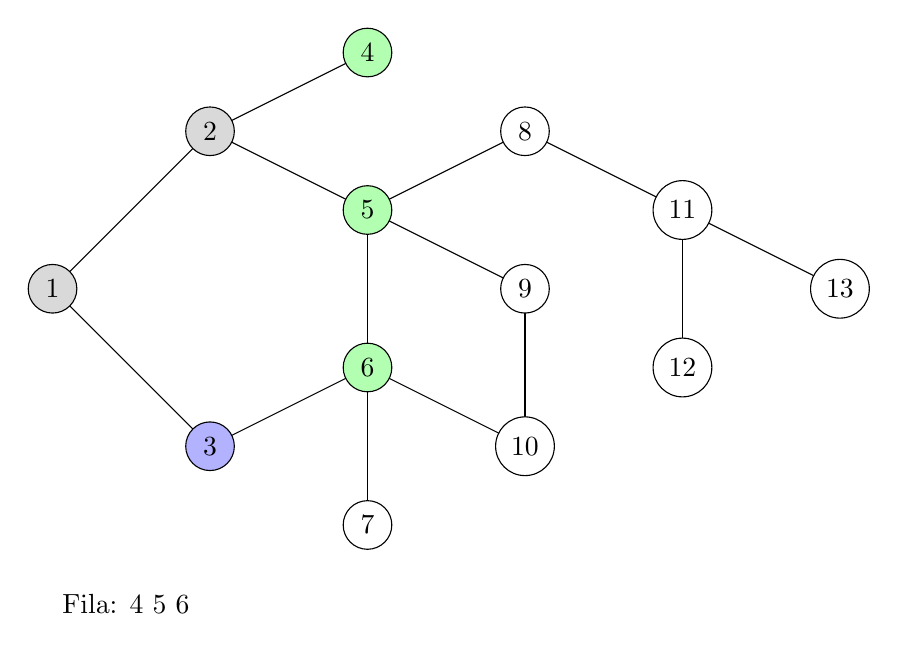
\begin{tikzpicture}
        \node[anchor=west] at (0,0) { Fila: 4 5 6 };
        \draw (0,4) -- (2,6);
        \draw (0,4) -- (2,2);
        \draw (2,6) -- (4,7);
        \draw (2,6) -- (4,5);
        \draw (4,5) -- (4,3);
        \draw (4,3) -- (2,2);
        \draw (4,3) -- (4,1);
        \draw (4,3) -- (6,2);
        \draw (4,5) -- (6,6);
        \draw (4,5) -- (6,4);
        \draw (6,2) -- (6,4);
        \draw (6,6) -- (8,5);
        \draw (8,5) -- (8,3);
        \draw (8,5) -- (10,4);

        \node[circle, draw, fill=gray!30] at (0, 4) {1};
        \node[circle, draw, fill=gray!30] at (2, 6) {2};
        \node[circle, draw, fill=blue!30] at (2, 2) {3};
        \node[circle, draw, fill=green!30] at (4, 7) {4};
        \node[circle, draw, fill=green!30] at (4, 5) {5};
        \node[circle, draw, fill=green!30] at (4, 3) {6};
        \node[circle, draw, fill=white] at (4, 1) {7};
        \node[circle, draw, fill=white] at (6, 6) {8};
        \node[circle, draw, fill=white] at (6, 4) {9};
        \node[circle, draw, fill=white] at (6, 2) {10};
        \node[circle, draw, fill=white] at (8, 5) {11};
        \node[circle, draw, fill=white] at (8, 3) {12};
        \node[circle, draw, fill=white] at (10, 4) {13};

    \end{tikzpicture}

\end{frame}

\begin{frame}[fragile]{Visualização da BFS}

    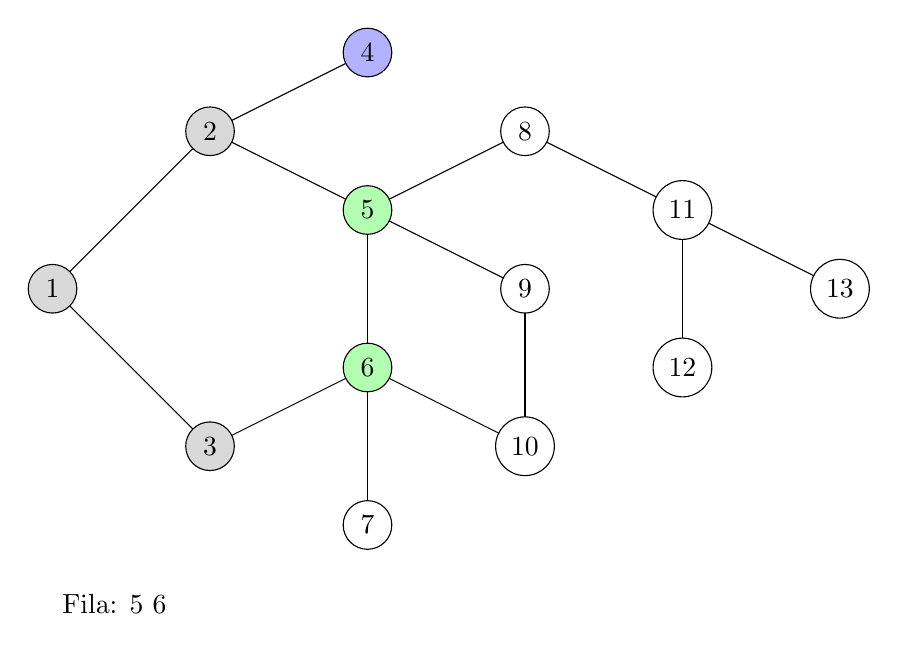
\begin{tikzpicture}
        \node[anchor=west] at (0,0) { Fila: 5 6 };
        \draw (0,4) -- (2,6);
        \draw (0,4) -- (2,2);
        \draw (2,6) -- (4,7);
        \draw (2,6) -- (4,5);
        \draw (4,5) -- (4,3);
        \draw (4,3) -- (2,2);
        \draw (4,3) -- (4,1);
        \draw (4,3) -- (6,2);
        \draw (4,5) -- (6,6);
        \draw (4,5) -- (6,4);
        \draw (6,2) -- (6,4);
        \draw (6,6) -- (8,5);
        \draw (8,5) -- (8,3);
        \draw (8,5) -- (10,4);

        \node[circle, draw, fill=gray!30] at (0, 4) {1};
        \node[circle, draw, fill=gray!30] at (2, 6) {2};
        \node[circle, draw, fill=gray!30] at (2, 2) {3};
        \node[circle, draw, fill=blue!30] at (4, 7) {4};
        \node[circle, draw, fill=green!30] at (4, 5) {5};
        \node[circle, draw, fill=green!30] at (4, 3) {6};
        \node[circle, draw, fill=white] at (4, 1) {7};
        \node[circle, draw, fill=white] at (6, 6) {8};
        \node[circle, draw, fill=white] at (6, 4) {9};
        \node[circle, draw, fill=white] at (6, 2) {10};
        \node[circle, draw, fill=white] at (8, 5) {11};
        \node[circle, draw, fill=white] at (8, 3) {12};
        \node[circle, draw, fill=white] at (10, 4) {13};

    \end{tikzpicture}

\end{frame}

\begin{frame}[fragile]{Visualização da BFS}

    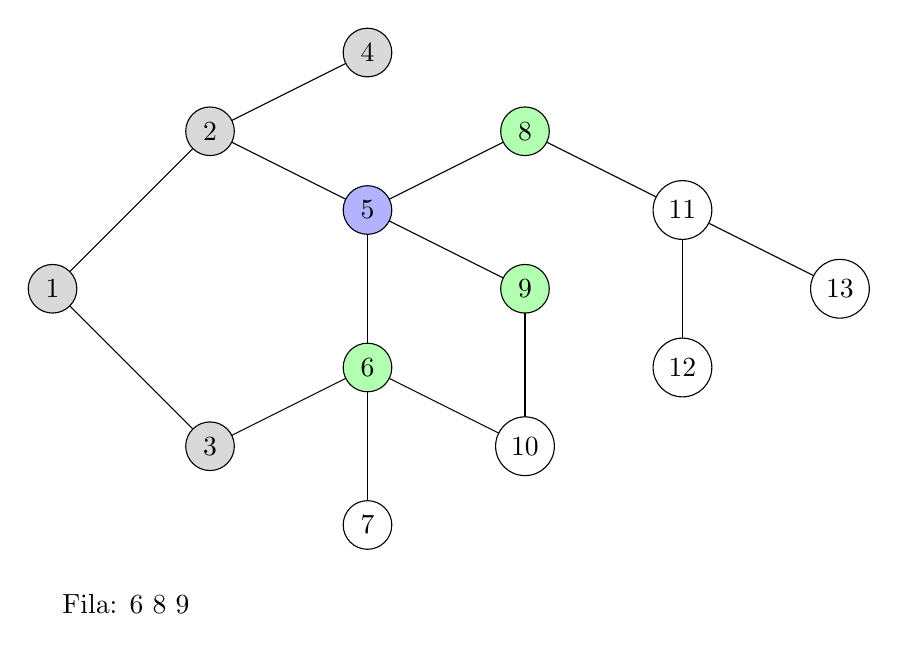
\begin{tikzpicture}
        \node[anchor=west] at (0,0) { Fila: 6 8 9 };
        \draw (0,4) -- (2,6);
        \draw (0,4) -- (2,2);
        \draw (2,6) -- (4,7);
        \draw (2,6) -- (4,5);
        \draw (4,5) -- (4,3);
        \draw (4,3) -- (2,2);
        \draw (4,3) -- (4,1);
        \draw (4,3) -- (6,2);
        \draw (4,5) -- (6,6);
        \draw (4,5) -- (6,4);
        \draw (6,2) -- (6,4);
        \draw (6,6) -- (8,5);
        \draw (8,5) -- (8,3);
        \draw (8,5) -- (10,4);

        \node[circle, draw, fill=gray!30] at (0, 4) {1};
        \node[circle, draw, fill=gray!30] at (2, 6) {2};
        \node[circle, draw, fill=gray!30] at (2, 2) {3};
        \node[circle, draw, fill=gray!30] at (4, 7) {4};
        \node[circle, draw, fill=blue!30] at (4, 5) {5};
        \node[circle, draw, fill=green!30] at (4, 3) {6};
        \node[circle, draw, fill=white] at (4, 1) {7};
        \node[circle, draw, fill=green!30] at (6, 6) {8};
        \node[circle, draw, fill=green!30] at (6, 4) {9};
        \node[circle, draw, fill=white] at (6, 2) {10};
        \node[circle, draw, fill=white] at (8, 5) {11};
        \node[circle, draw, fill=white] at (8, 3) {12};
        \node[circle, draw, fill=white] at (10, 4) {13};

    \end{tikzpicture}

\end{frame}

\begin{frame}[fragile]{Visualização da BFS}

    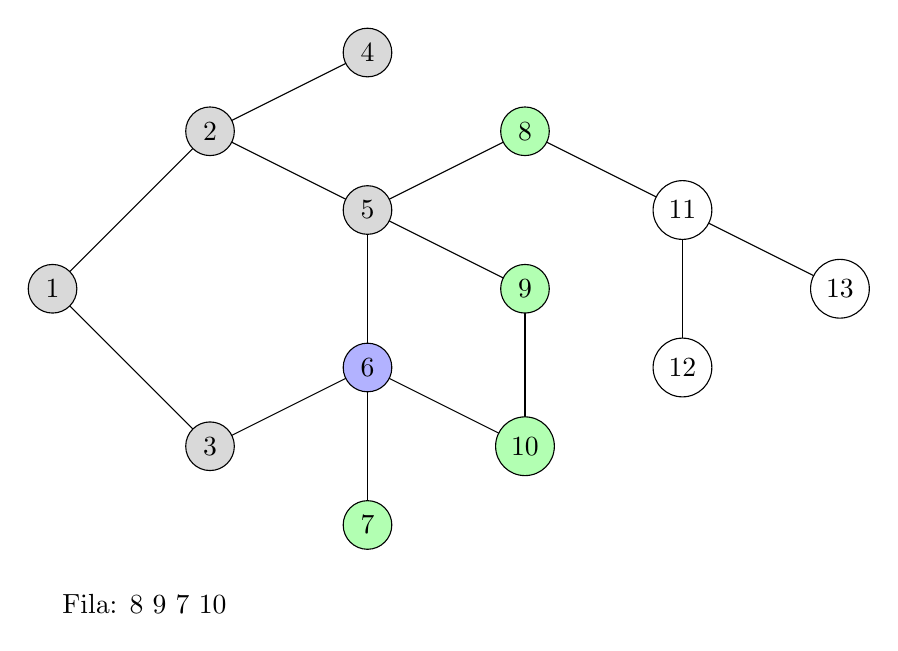
\begin{tikzpicture}
        \node[anchor=west] at (0,0) { Fila: 8 9 7 10 };
        \draw (0,4) -- (2,6);
        \draw (0,4) -- (2,2);
        \draw (2,6) -- (4,7);
        \draw (2,6) -- (4,5);
        \draw (4,5) -- (4,3);
        \draw (4,3) -- (2,2);
        \draw (4,3) -- (4,1);
        \draw (4,3) -- (6,2);
        \draw (4,5) -- (6,6);
        \draw (4,5) -- (6,4);
        \draw (6,2) -- (6,4);
        \draw (6,6) -- (8,5);
        \draw (8,5) -- (8,3);
        \draw (8,5) -- (10,4);

        \node[circle, draw, fill=gray!30] at (0, 4) {1};
        \node[circle, draw, fill=gray!30] at (2, 6) {2};
        \node[circle, draw, fill=gray!30] at (2, 2) {3};
        \node[circle, draw, fill=gray!30] at (4, 7) {4};
        \node[circle, draw, fill=gray!30] at (4, 5) {5};
        \node[circle, draw, fill=blue!30] at (4, 3) {6};
        \node[circle, draw, fill=green!30] at (4, 1) {7};
        \node[circle, draw, fill=green!30] at (6, 6) {8};
        \node[circle, draw, fill=green!30] at (6, 4) {9};
        \node[circle, draw, fill=green!30] at (6, 2) {10};
        \node[circle, draw, fill=white] at (8, 5) {11};
        \node[circle, draw, fill=white] at (8, 3) {12};
        \node[circle, draw, fill=white] at (10, 4) {13};

    \end{tikzpicture}

\end{frame}

\begin{frame}[fragile]{Visualização da BFS}

    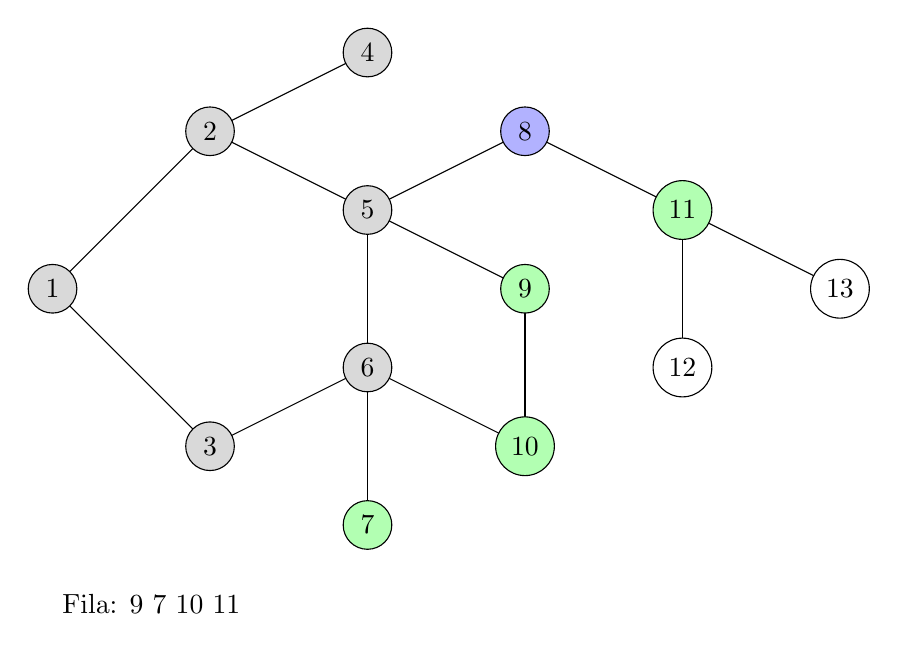
\begin{tikzpicture}
        \node[anchor=west] at (0,0) { Fila: 9 7 10 11 };
        \draw (0,4) -- (2,6);
        \draw (0,4) -- (2,2);
        \draw (2,6) -- (4,7);
        \draw (2,6) -- (4,5);
        \draw (4,5) -- (4,3);
        \draw (4,3) -- (2,2);
        \draw (4,3) -- (4,1);
        \draw (4,3) -- (6,2);
        \draw (4,5) -- (6,6);
        \draw (4,5) -- (6,4);
        \draw (6,2) -- (6,4);
        \draw (6,6) -- (8,5);
        \draw (8,5) -- (8,3);
        \draw (8,5) -- (10,4);

        \node[circle, draw, fill=gray!30] at (0, 4) {1};
        \node[circle, draw, fill=gray!30] at (2, 6) {2};
        \node[circle, draw, fill=gray!30] at (2, 2) {3};
        \node[circle, draw, fill=gray!30] at (4, 7) {4};
        \node[circle, draw, fill=gray!30] at (4, 5) {5};
        \node[circle, draw, fill=gray!30] at (4, 3) {6};
        \node[circle, draw, fill=green!30] at (4, 1) {7};
        \node[circle, draw, fill=blue!30] at (6, 6) {8};
        \node[circle, draw, fill=green!30] at (6, 4) {9};
        \node[circle, draw, fill=green!30] at (6, 2) {10};
        \node[circle, draw, fill=green!30] at (8, 5) {11};
        \node[circle, draw, fill=white] at (8, 3) {12};
        \node[circle, draw, fill=white] at (10, 4) {13};

    \end{tikzpicture}

\end{frame}

\begin{frame}[fragile]{Visualização da BFS}

    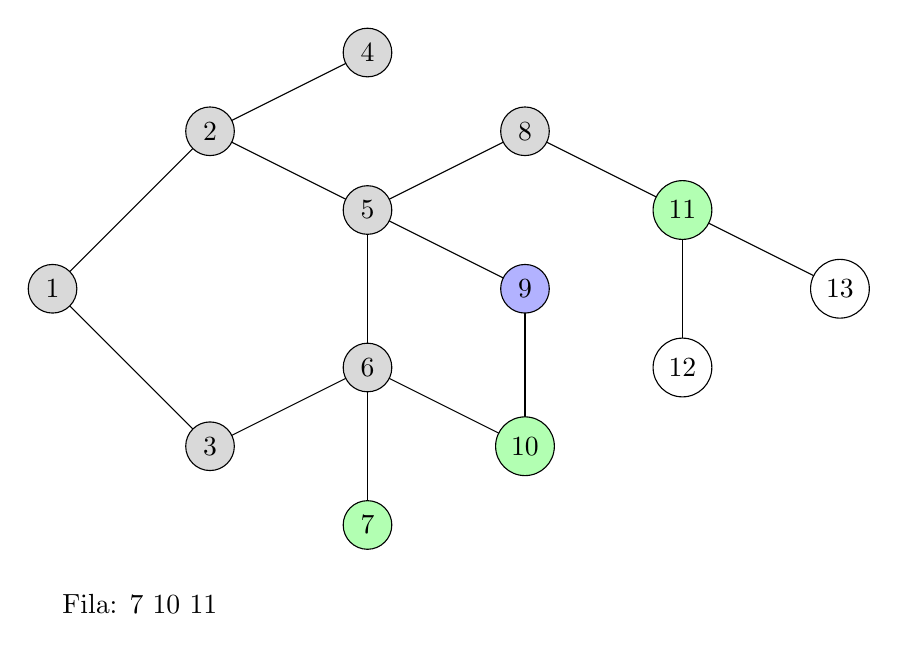
\begin{tikzpicture}
        \node[anchor=west] at (0,0) { Fila: 7 10 11 };
        \draw (0,4) -- (2,6);
        \draw (0,4) -- (2,2);
        \draw (2,6) -- (4,7);
        \draw (2,6) -- (4,5);
        \draw (4,5) -- (4,3);
        \draw (4,3) -- (2,2);
        \draw (4,3) -- (4,1);
        \draw (4,3) -- (6,2);
        \draw (4,5) -- (6,6);
        \draw (4,5) -- (6,4);
        \draw (6,2) -- (6,4);
        \draw (6,6) -- (8,5);
        \draw (8,5) -- (8,3);
        \draw (8,5) -- (10,4);

        \node[circle, draw, fill=gray!30] at (0, 4) {1};
        \node[circle, draw, fill=gray!30] at (2, 6) {2};
        \node[circle, draw, fill=gray!30] at (2, 2) {3};
        \node[circle, draw, fill=gray!30] at (4, 7) {4};
        \node[circle, draw, fill=gray!30] at (4, 5) {5};
        \node[circle, draw, fill=gray!30] at (4, 3) {6};
        \node[circle, draw, fill=green!30] at (4, 1) {7};
        \node[circle, draw, fill=gray!30] at (6, 6) {8};
        \node[circle, draw, fill=blue!30] at (6, 4) {9};
        \node[circle, draw, fill=green!30] at (6, 2) {10};
        \node[circle, draw, fill=green!30] at (8, 5) {11};
        \node[circle, draw, fill=white] at (8, 3) {12};
        \node[circle, draw, fill=white] at (10, 4) {13};

    \end{tikzpicture}

\end{frame}

\begin{frame}[fragile]{Visualização da BFS}

    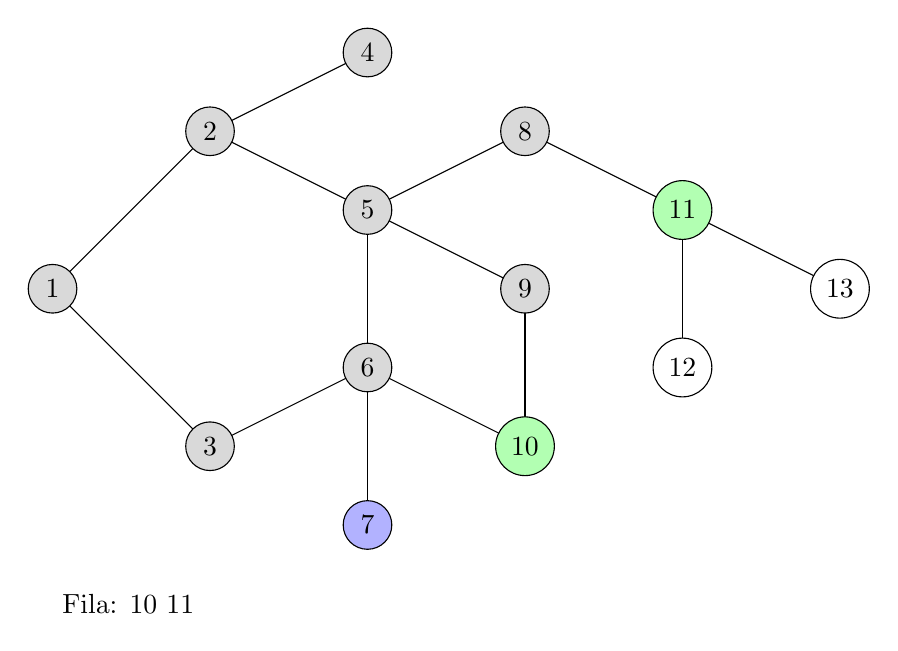
\begin{tikzpicture}
        \node[anchor=west] at (0,0) { Fila: 10 11 };
        \draw (0,4) -- (2,6);
        \draw (0,4) -- (2,2);
        \draw (2,6) -- (4,7);
        \draw (2,6) -- (4,5);
        \draw (4,5) -- (4,3);
        \draw (4,3) -- (2,2);
        \draw (4,3) -- (4,1);
        \draw (4,3) -- (6,2);
        \draw (4,5) -- (6,6);
        \draw (4,5) -- (6,4);
        \draw (6,2) -- (6,4);
        \draw (6,6) -- (8,5);
        \draw (8,5) -- (8,3);
        \draw (8,5) -- (10,4);

        \node[circle, draw, fill=gray!30] at (0, 4) {1};
        \node[circle, draw, fill=gray!30] at (2, 6) {2};
        \node[circle, draw, fill=gray!30] at (2, 2) {3};
        \node[circle, draw, fill=gray!30] at (4, 7) {4};
        \node[circle, draw, fill=gray!30] at (4, 5) {5};
        \node[circle, draw, fill=gray!30] at (4, 3) {6};
        \node[circle, draw, fill=blue!30] at (4, 1) {7};
        \node[circle, draw, fill=gray!30] at (6, 6) {8};
        \node[circle, draw, fill=gray!30] at (6, 4) {9};
        \node[circle, draw, fill=green!30] at (6, 2) {10};
        \node[circle, draw, fill=green!30] at (8, 5) {11};
        \node[circle, draw, fill=white] at (8, 3) {12};
        \node[circle, draw, fill=white] at (10, 4) {13};

    \end{tikzpicture}

\end{frame}

\begin{frame}[fragile]{Visualização da BFS}

    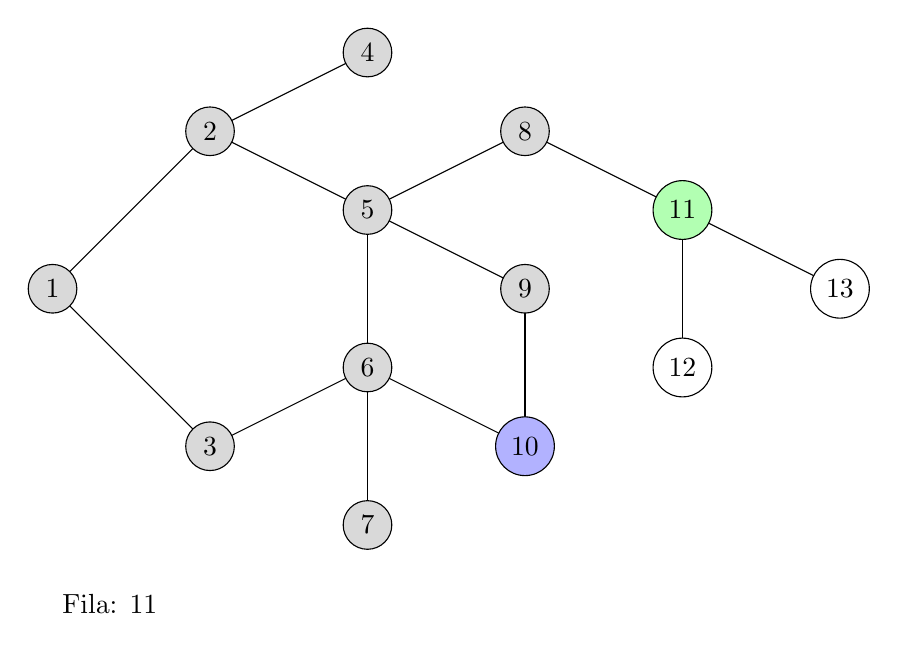
\begin{tikzpicture}
        \node[anchor=west] at (0,0) { Fila: 11 };
        \draw (0,4) -- (2,6);
        \draw (0,4) -- (2,2);
        \draw (2,6) -- (4,7);
        \draw (2,6) -- (4,5);
        \draw (4,5) -- (4,3);
        \draw (4,3) -- (2,2);
        \draw (4,3) -- (4,1);
        \draw (4,3) -- (6,2);
        \draw (4,5) -- (6,6);
        \draw (4,5) -- (6,4);
        \draw (6,2) -- (6,4);
        \draw (6,6) -- (8,5);
        \draw (8,5) -- (8,3);
        \draw (8,5) -- (10,4);

        \node[circle, draw, fill=gray!30] at (0, 4) {1};
        \node[circle, draw, fill=gray!30] at (2, 6) {2};
        \node[circle, draw, fill=gray!30] at (2, 2) {3};
        \node[circle, draw, fill=gray!30] at (4, 7) {4};
        \node[circle, draw, fill=gray!30] at (4, 5) {5};
        \node[circle, draw, fill=gray!30] at (4, 3) {6};
        \node[circle, draw, fill=gray!30] at (4, 1) {7};
        \node[circle, draw, fill=gray!30] at (6, 6) {8};
        \node[circle, draw, fill=gray!30] at (6, 4) {9};
        \node[circle, draw, fill=blue!30] at (6, 2) {10};
        \node[circle, draw, fill=green!30] at (8, 5) {11};
        \node[circle, draw, fill=white] at (8, 3) {12};
        \node[circle, draw, fill=white] at (10, 4) {13};

    \end{tikzpicture}

\end{frame}

\begin{frame}[fragile]{Visualização da BFS}

    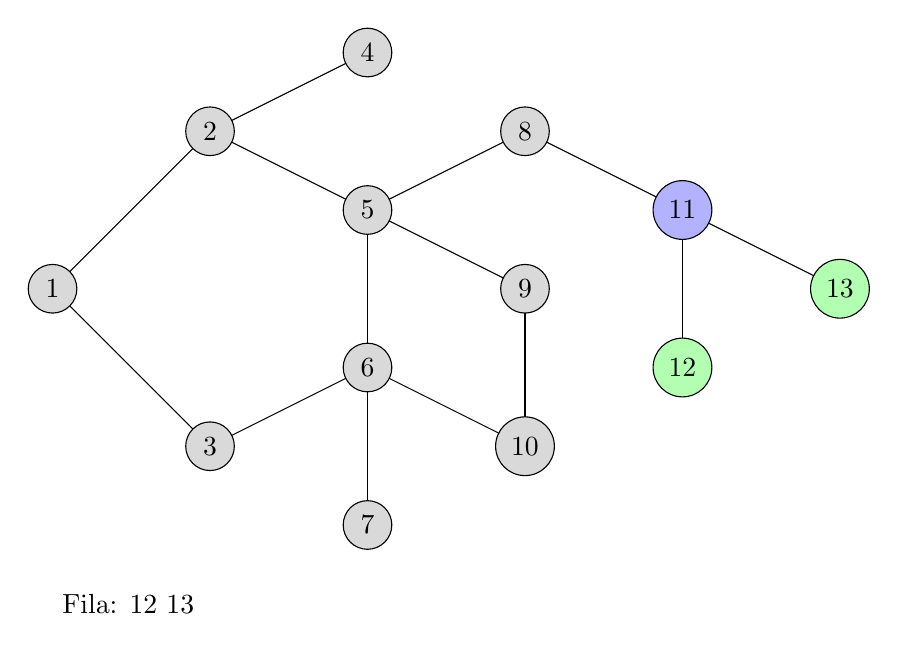
\begin{tikzpicture}
        \node[anchor=west] at (0,0) { Fila: 12 13 };
        \draw (0,4) -- (2,6);
        \draw (0,4) -- (2,2);
        \draw (2,6) -- (4,7);
        \draw (2,6) -- (4,5);
        \draw (4,5) -- (4,3);
        \draw (4,3) -- (2,2);
        \draw (4,3) -- (4,1);
        \draw (4,3) -- (6,2);
        \draw (4,5) -- (6,6);
        \draw (4,5) -- (6,4);
        \draw (6,2) -- (6,4);
        \draw (6,6) -- (8,5);
        \draw (8,5) -- (8,3);
        \draw (8,5) -- (10,4);

        \node[circle, draw, fill=gray!30] at (0, 4) {1};
        \node[circle, draw, fill=gray!30] at (2, 6) {2};
        \node[circle, draw, fill=gray!30] at (2, 2) {3};
        \node[circle, draw, fill=gray!30] at (4, 7) {4};
        \node[circle, draw, fill=gray!30] at (4, 5) {5};
        \node[circle, draw, fill=gray!30] at (4, 3) {6};
        \node[circle, draw, fill=gray!30] at (4, 1) {7};
        \node[circle, draw, fill=gray!30] at (6, 6) {8};
        \node[circle, draw, fill=gray!30] at (6, 4) {9};
        \node[circle, draw, fill=gray!30] at (6, 2) {10};
        \node[circle, draw, fill=blue!30] at (8, 5) {11};
        \node[circle, draw, fill=green!30] at (8, 3) {12};
        \node[circle, draw, fill=green!30] at (10, 4) {13};

    \end{tikzpicture}

\end{frame}

\begin{frame}[fragile]{Visualização da BFS}

    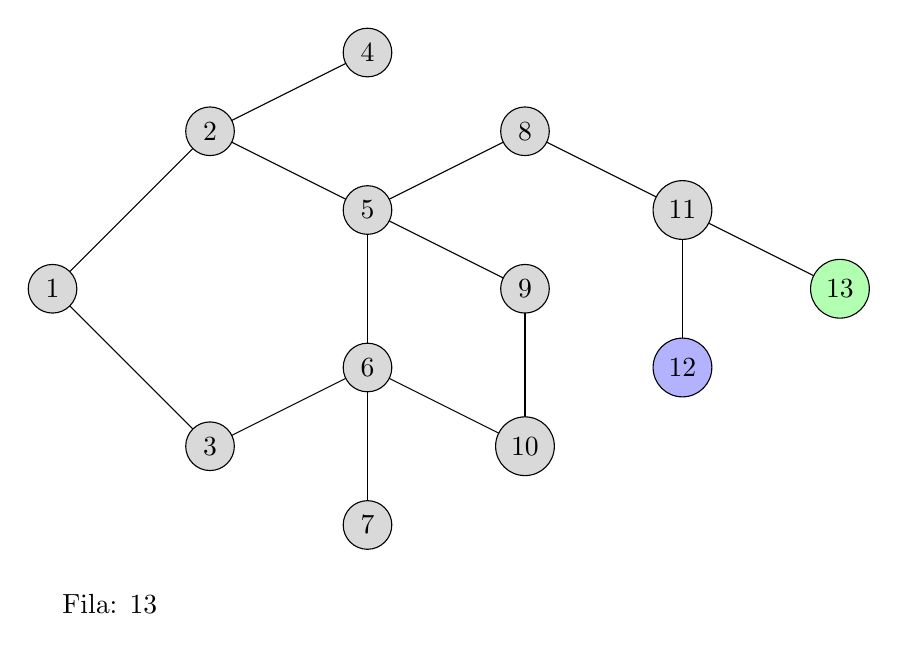
\begin{tikzpicture}
        \node[anchor=west] at (0,0) { Fila: 13 };
        \draw (0,4) -- (2,6);
        \draw (0,4) -- (2,2);
        \draw (2,6) -- (4,7);
        \draw (2,6) -- (4,5);
        \draw (4,5) -- (4,3);
        \draw (4,3) -- (2,2);
        \draw (4,3) -- (4,1);
        \draw (4,3) -- (6,2);
        \draw (4,5) -- (6,6);
        \draw (4,5) -- (6,4);
        \draw (6,2) -- (6,4);
        \draw (6,6) -- (8,5);
        \draw (8,5) -- (8,3);
        \draw (8,5) -- (10,4);

        \node[circle, draw, fill=gray!30] at (0, 4) {1};
        \node[circle, draw, fill=gray!30] at (2, 6) {2};
        \node[circle, draw, fill=gray!30] at (2, 2) {3};
        \node[circle, draw, fill=gray!30] at (4, 7) {4};
        \node[circle, draw, fill=gray!30] at (4, 5) {5};
        \node[circle, draw, fill=gray!30] at (4, 3) {6};
        \node[circle, draw, fill=gray!30] at (4, 1) {7};
        \node[circle, draw, fill=gray!30] at (6, 6) {8};
        \node[circle, draw, fill=gray!30] at (6, 4) {9};
        \node[circle, draw, fill=gray!30] at (6, 2) {10};
        \node[circle, draw, fill=gray!30] at (8, 5) {11};
        \node[circle, draw, fill=blue!30] at (8, 3) {12};
        \node[circle, draw, fill=green!30] at (10, 4) {13};

    \end{tikzpicture}

\end{frame}

\begin{frame}[fragile]{Visualização da BFS}

    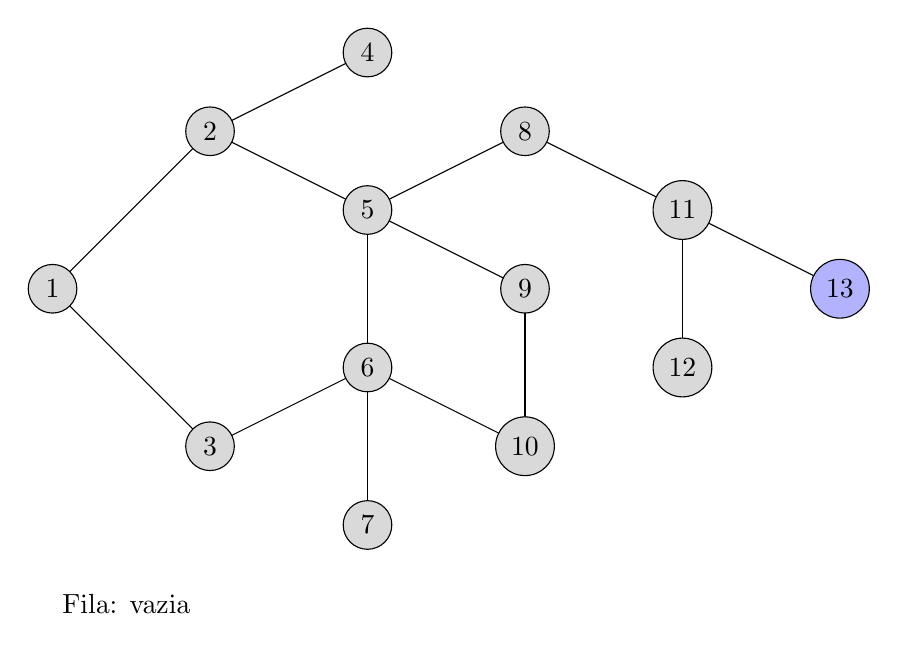
\begin{tikzpicture}
        \node[anchor=west] at (0,0) { Fila: vazia };
        \draw (0,4) -- (2,6);
        \draw (0,4) -- (2,2);
        \draw (2,6) -- (4,7);
        \draw (2,6) -- (4,5);
        \draw (4,5) -- (4,3);
        \draw (4,3) -- (2,2);
        \draw (4,3) -- (4,1);
        \draw (4,3) -- (6,2);
        \draw (4,5) -- (6,6);
        \draw (4,5) -- (6,4);
        \draw (6,2) -- (6,4);
        \draw (6,6) -- (8,5);
        \draw (8,5) -- (8,3);
        \draw (8,5) -- (10,4);

        \node[circle, draw, fill=gray!30] at (0, 4) {1};
        \node[circle, draw, fill=gray!30] at (2, 6) {2};
        \node[circle, draw, fill=gray!30] at (2, 2) {3};
        \node[circle, draw, fill=gray!30] at (4, 7) {4};
        \node[circle, draw, fill=gray!30] at (4, 5) {5};
        \node[circle, draw, fill=gray!30] at (4, 3) {6};
        \node[circle, draw, fill=gray!30] at (4, 1) {7};
        \node[circle, draw, fill=gray!30] at (6, 6) {8};
        \node[circle, draw, fill=gray!30] at (6, 4) {9};
        \node[circle, draw, fill=gray!30] at (6, 2) {10};
        \node[circle, draw, fill=gray!30] at (8, 5) {11};
        \node[circle, draw, fill=gray!30] at (8, 3) {12};
        \node[circle, draw, fill=blue!30] at (10, 4) {13};

    \end{tikzpicture}

\end{frame}

